\documentclass{article}

\usepackage{PRIMEarxiv}

\usepackage[utf8]{inputenc}
\usepackage[T1]{fontenc}
\usepackage{hyperref}
\usepackage{url}
\usepackage{xurl}
\usepackage{booktabs}
\usepackage{amsfonts}
\usepackage{microtype}
\usepackage{amsmath}
\usepackage{graphicx}
\usepackage{tabularx}
\usepackage{array}
\usepackage{float}
\usepackage{listings}
\usepackage{tikz}
\usetikzlibrary{shapes.geometric, arrows.meta, positioning, calc, fit, backgrounds, shadows}
\lstset{basicstyle=\ttfamily, breaklines=true}


% Define a custom column type for ragged-right text in tabularx
\newcolumntype{L}{>{\raggedright\arraybackslash}X}

%% Title from verigov.html
\title{VeriGov: A Crypto-Economic Protocol for Decentralized Software Supply Chain Security}

\author{
  Nikhil Ranjan \\
  \texttt{nikhil@polkassembly.io} \\
}

\begin{document}
\maketitle

\begin{abstract}
The proliferation of open-source software has created a complex and vulnerable software supply chain, where centralized trust in repositories and developers has become a significant liability. Recent attacks demonstrate that current security measures, such as checksums and basic code signing, are insufficient to prevent the distribution of malicious or tampered software. These mechanisms fail to provide two critical guarantees: \emph{provenance integrity} (a verifiable link from source code to binary) and \emph{release authorization integrity} (assurance that a release was approved by a legitimate, collective consensus). This paper introduces VeriGov, a crypto-economic protocol that addresses these gaps by establishing a Decentralized Autonomous Organization (DAO) to govern the software release lifecycle. VeriGov leverages a public, permissionless blockchain to create an immutable, auditable ledger for release management. Inspired by Polkadot's on-chain governance, it establishes a multi-stakeholder system where release approvals are subject to a configurable $m$-of-$n$ vote, weighted by staked holdings of the native utility token, \texttt{VGOV}. Furthermore, VeriGov incorporates cryptographic attestations from reproducible build processes to create a non-repudiable link between a software binary and its corresponding source code. This paper details the protocol's architecture, its DAO-based governance for release and stakeholder management, and its tokenomic model, which uses staking and slashing mechanisms---including separately-adjudicated negligence and malice slashing---to create economic incentives for security and trust.
\end{abstract}

\section{Introduction}
\label{sec:introduction}

\subsection{Open Source as Critical Infrastructure}

The modern digital infrastructure is built upon a foundation of open-source software (OSS). The collaborative and transparent nature of OSS development has accelerated innovation at an unprecedented scale, but the same openness has also turned the software supply chain into one of the most attractive attack surfaces in computing. Modern applications are not monolithic entities but are composed of vast and intricate dependency trees, often pulling in hundreds or even thousands of third-party components.~\cite{ohm2020backstabber} A single vulnerability or malicious component introduced anywhere in this complex web can propagate downstream, creating a cascading failure with devastating consequences.~\cite{ladisa2023sok} The widespread deployment of this software on millions of devices, coupled with the prevalence of automatic update mechanisms, transforms this interconnectedness into a vast and attractive attack surface for malicious actors.~\cite{nhtsa2020firmware}

\subsection{The Centralized Trust Crisis}

Despite the decentralized ethos of the open-source community, the infrastructure that supports it remains critically centralized. Package registries like npm and PyPI, and source code repositories such as GitHub, act as central points of trust and control. The authority to publish or modify a package is often concentrated in the hands of a single repository owner or a small, insular group of maintainers.~\cite{aikido2025rand} This centralization represents a fundamental architectural vulnerability. The infamous SolarWinds attack, where a compromise of the build system led to the distribution of malicious updates to over 18,000 organizations, serves as a stark reminder of the risks inherent in placing trust in a single vendor or a single point in the supply chain.~\cite{cisa2020solarwinds} When the security of a global ecosystem hinges on the security practices and integrity of a few individuals or systems, the model itself becomes the primary risk.

\subsection{Illustrative Catastrophes: The Evolving Threat}

The theoretical risks of this centralized trust model have been realized in numerous high-profile attacks, which demonstrate an evolving threat landscape that targets different stages of the software lifecycle.

In one model, an external adversary compromises a weak link in the chain. The May 2025 attack on the \lstinline{rand-user-agent} npm package is a canonical example. An attacker utilized a stolen, outdated, and insufficiently secured automation token to publish malicious versions of the package directly to the npm registry. Crucially, these malicious versions had no corresponding source code commits in the project's official GitHub repository.~\cite{aikido2025rand} This incident starkly illustrates the dangerous disconnect between the perceived source of truth (the code repository) and the actual distribution channel (the package registry). The checksums provided by npm would correctly verify the integrity of the downloaded malicious package, but they offer no assurance that the package was derived from the trusted source code.

A more insidious threat model involves the trusted insider. In March 2022, the legitimate maintainer of node-ipc, a package with over a million weekly downloads, intentionally introduced malicious code into new versions. This "protestware" was designed to target users based on their geolocation, specifically wiping files on systems in Russia and Belarus with a heart emoji to protest the war in Ukraine.~\cite{cve-2022-23812} This attack vector is particularly pernicious because it bypasses all traditional authentication mechanisms. The maintainer's identity was correct, their credentials were not compromised, and they had the legitimate authority to publish the package. The failure was not one of authentication but of trust and intent. The 2024 \lstinline{xz-utils} backdoor (CVE-2024-3094) further escalated this threat model: a multi-year social-engineering campaign cultivated a maintainer position in a foundational compression library and inserted an SSH backdoor smuggled inside binary test fixtures, undetectable by source code review of the upstream repository.~\cite{freund2024xz,cve-2024-3094} These incidents prove that security models based solely on authenticating the identity of a single developer are fundamentally flawed in the face of a malicious, coerced, or long-game adversarial insider.

\subsection{The Fundamental Trust Gaps}

These incidents expose two critical gaps in the security of the modern software supply chain, which this paper aims to address:

\begin{enumerate}
\item \textbf{The Provenance Gap:} There is no standard, cryptographically verifiable mechanism for an end-user to confirm that a binary artifact they have downloaded was produced by the specific, publicly visible source code it claims to represent. A checksum verifies that the bits downloaded are the same as the bits uploaded to the server, but it provides no guarantee about the origin or the process that created those bits.~\cite{lamb2022reproducible}
\item \textbf{The Authorization Gap:} There is no mechanism to verify that a release was the result of a legitimate, collective decision-making process. The approval of a release is an opaque, off-chain process. Consequently, a single point of compromise---whether it is a stolen developer credential, a compromised build server, or a malicious insider---is sufficient to authorize and distribute a malicious update to the entire user base.~\cite{aikido2025rand}
\end{enumerate}

The evolution of threats from simple data corruption to sophisticated attacks targeting developer intent necessitates a paradigm shift. Initial security measures focused on preventing unauthorized changes (e.g., checksums). This evolved to authenticating the source of the change (e.g., GPG signing). Attacks like \lstinline{rand-user-agent} revealed that even an "authentic" credential could be misused, highlighting a process failure between development and distribution. The \lstinline{node-ipc} attack represents a further maturation of the threat, where the identity is correct and the credentials are secure, but the intent of the trusted actor is malicious. This demonstrates that trusting any single actor, no matter how well-authenticated, is an insufficient security model. The security paradigm must therefore evolve from authenticating a single actor's identity to verifying a collective, multi-stakeholder decision. This requires a move away from centralized trust models towards a trustless, permissionless protocol governed by a DAO and secured by crypto-economic incentives.~\cite{wright2015decentralized}

\subsection{Thesis and Contribution}

This paper proposes VeriGov, a decentralized crypto-economic protocol designed to close the provenance and authorization gaps in the software supply chain. VeriGov integrates concepts from distributed ledger technology, on-chain governance, and verifiable build systems to create a resilient and transparent ecosystem for software distribution and updates.

The primary contributions of this work are:

\begin{enumerate}
\item A decentralized, on-chain governance protocol, inspired by Polkadot's OpenGov, that requires multi-stakeholder approval for software releases via a configurable cryptographic voting mechanism, weighted by staked tokens.
\item A protocol for generating and verifying a cryptographic attestation that creates a non-repudiable, verifiable link between a specific version of the source code and its compiled binary artifact.
\item A comprehensive protocol architecture that combines these elements to provide end-to-end security, from source code to end-user device.
\item A novel tokenomic model, centered around the \lstinline{VGOV} token, that aligns incentives and secures the protocol through staking and slashing mechanisms.
\end{enumerate}

This paper will proceed by first providing a formal analysis of the threat landscape, followed by a critical review of existing solutions. It will then detail the VeriGov architecture and its core protocols, and conclude with a rigorous security analysis against the identified threats.

\section{The Software Supply Chain Threat Model}
\label{sec:the-software-supply-chain-threat-model}

A comprehensive defense requires a systematic understanding of the adversary's methods. The software supply chain is not a single entity but a complex graph of dependencies, tools, and human actors, each presenting a potential attack vector. Recent surveys provide systematic taxonomies of attacks on open-source supply chains and demonstrate the structural fragility of large package ecosystems.~\cite{ladisa2023sok,ohm2020backstabber,zimmermann2019small,duan2021measuring} This section synthesizes these results with recent real-world incidents to motivate the security properties VeriGov is designed to provide.

\subsection{A Systematic Review of Attack Vectors}

The attack vectors can be broadly categorized based on the point of compromise within the supply chain. These categories are not mutually exclusive and are often combined by attackers to form a sophisticated kill chain.

\subsubsection{Package Registry Attacks}

These attacks target the public repositories that developers and build systems trust to fetch dependencies.

\begin{itemize}
\item \textbf{Typosquatting:} This technique relies on simple human error. Attackers publish malicious packages with names that are common misspellings or typographical variations of popular, legitimate packages. For instance, a developer intending to install \lstinline{request} might accidentally type \lstinline{reqeust}. Examples include the malicious \lstinline{express-cookie-parser} imitating the popular \lstinline{cookie-parser} library, and \lstinline{xlsx-to-json-lh} impersonating \lstinline{xlsx-to-json-lc}.~\cite{ohm2020backstabber} This vector has proven remarkably effective due to its simplicity and the high volume of package installations in typical development workflows.~\cite{zimmermann2019small}
\item \textbf{Dependency Confusion:} A more advanced attack, dependency confusion targets organizations that use a mix of private, internal package repositories and public ones like npm or PyPI. An attacker first discovers the names of internal packages (which may leak through public code snippets or configuration files). They then publish a malicious package with the same name to a public repository, but assign it a much higher version number (e.g., \lstinline{99.9.9}). When a developer's package manager or an automated build system is configured to resolve dependencies, it may see the higher-versioned public package and "confuse" it for a legitimate update to the internal one, thereby pulling and executing the malicious code.~\cite{ohm2020backstabber} This attack vector exploits the default behaviors of many package managers, which prioritize the newest available version of a package regardless of its source.~\cite{ohm2020backstabber}
\end{itemize}

\subsubsection{Upstream Compromise}

These attacks target the assets and infrastructure of the open-source project itself, further up the supply chain.

\begin{itemize}
\item \textbf{Maintainer Account Takeover:} Attackers actively target the credentials of legitimate package maintainers through phishing, social engineering, or by exploiting weak authentication practices. Once an attacker gains control of a maintainer's account or an associated automation token, they can publish malicious updates to trusted packages that are then automatically consumed by thousands of downstream projects.~\cite{ohm2020backstabber} The \lstinline{rand-user-agent} incident, where an attacker leveraged a compromised and outdated npm automation token that was not protected by two-factor authentication, is a perfect illustration of this threat.~\cite{aikido2025rand}
\item \textbf{Source Code Injection:} This involves directly compromising the project's source code repository (e.g., GitHub) or, more commonly, an individual developer's workstation. By injecting malicious code into the source, the attacker ensures that the malicious logic becomes a permanent part of the project's history. Securing developer workstations and the development platform itself is critical to mitigating this threat, as these environments are often less controlled and can be a gateway for attackers to alter code, introduce backdoors, and steal intellectual property.~\cite{ladisa2023sok}
\item \textbf{Build/CI/CD Pipeline Compromise:} This is one of the most dangerous attack vectors because it can be invisible to developers reviewing the source code. An attacker who compromises the build server or the continuous integration/continuous deployment (CI/CD) pipeline can inject malicious code directly into the binary artifacts during the compilation or packaging process. The source code in the repository remains clean, but the distributed software is compromised. The SolarWinds attack is the most prominent example of this technique, where attackers compromised the Orion Platform's build system to insert a backdoor into signed, legitimate-looking software updates.~\cite{cisa2020solarwinds}
\end{itemize}

\subsubsection{Malicious Maintainer and "Protestware"}

This category of threat challenges the very notion of a "trusted insider" and demonstrates that authentication alone is not security.

\begin{itemize}
\item \textbf{Intentional Sabotage:} A legitimate, authenticated maintainer with full authority over a project can choose to intentionally sabotage it. The \lstinline{node-ipc} incident is the canonical case, where the maintainer embedded destructive malware into the package as a form of political protest.~\cite{cve-2022-23812} A similar, though less destructive, incident involved the maintainer of \lstinline{colors.js} and \lstinline{faker.js} who intentionally pushed broken versions, causing widespread application failures.~\cite{ohm2020backstabber}
\item \textbf{"Protestware":} A growing trend involves developers using their software as a platform for activism. This can range from the destructive (\lstinline{node-ipc}) to the benign. For example, new versions of the popular \lstinline{styled-components} and \lstinline{es5-ext} packages were modified to detect if they were being installed on Russian systems and, if so, print anti-war messages to the console.~\cite{ohm2020backstabber} While the intent may not be traditionally malicious, this practice fundamentally undermines the trust contract between software producers and consumers. Users expect software to perform its stated function, not to serve as a vehicle for the developer's political views.~\cite{ladisa2023sok} This vector proves that even a perfectly authenticated identity cannot guarantee benign intent.
\end{itemize}

The combination of these vectors can form a sophisticated kill chain. An attacker could begin by using dependency confusion to gain an initial foothold, exfiltrating credentials from a compromised build environment.~\cite{birsan2021dependency} With these credentials, they could then access and modify the build pipeline, injecting a remote access trojan (RAT) into the final binary artifact, all without ever touching the public source code.~\cite{cisa2020solarwinds} The legitimate maintainer, unaware of the compromise, would then sign and publish this malicious binary, leveraging the project's established trust to distribute the malware. This scenario highlights that securing isolated components is insufficient; the entire lifecycle from dependency resolution to build and publication must be verifiable.

\subsection{Formal Problem Definition}

To rigorously address these threats, we formally define the security properties that are currently lacking in the software supply chain. Let $S$ be the source code of a project at a specific commit $c$, denoted $S_c$. Let $B$ be the resulting binary artifact. Let $H$ be a secure cryptographic hash function (e.g., SHA-256).

\begin{itemize}
\item \textbf{Provenance Integrity} ($P_I$): A system is said to provide provenance integrity if, for a given binary $B$ and source commit $c$, there exists a verifiable cryptographic attestation, $A_{build}$, that non-repudiably binds the hash of the source code, $H(S_c)$, to the hash of the binary, $H(B)$. This attestation must be generated as part of a trusted and verifiable build process.
$$P_I \iff \exists A_{build} : \text{verify}(A_{build}, H(S_c), H(B)) = \text{true}$$
Current systems largely fail to provide this. A user typically receives $B$ and a checksum $H(B)$, but this provides no cryptographic link back to the source code $S_c$ that supposedly produced it.

\item \textbf{Release Authorization Integrity} ($R_A$): Let $\{V_1, V_2,..., V_n\}$ be the set of public keys corresponding to the authorized stakeholders of a project. Let a release policy be defined by a threshold $m$ where $1 \le m \le n$. A system provides release authorization integrity if a release of binary $B$ is considered valid if and only if it is accompanied by a set of at least $m$ valid digital signatures, $\{\sigma_1, \sigma_2,..., \sigma_m\}$, where each $\sigma_i$ is a signature over $H(B)$ from a distinct stakeholder $V_i$.
$$R_A \iff \exists \{\sigma_{i_1},..., \sigma_{i_k}\} \text{ s.t. } k \ge m \land \forall j \in \{1,..., k\}, \text{verify\_sig}(V_{i_j}, H(B), \sigma_{i_j}) = \text{true}$$
Current systems fail this property, as a release can often be authorized by a single signature or a single compromised account ($m=1$), creating a single point of failure.~\cite{aikido2025rand}
\end{itemize}

\section{Related Work: A Critical Assessment of Existing Solutions}
\label{sec:related-work-a-critical-assessment-of-existing-s}

Several frameworks and technologies have been developed to address aspects of software supply chain security. However, as this section will demonstrate, they are incomplete solutions that fail to address the fundamental gaps of provenance and authorization integrity in a holistic manner.

\subsection{The Update Framework (TUF)}

The Update Framework (TUF) is a CNCF-graduated project designed to secure software update systems.~\cite{samuel2010tuf} Its primary contribution is providing compromise-resilience for the distribution channel.

\begin{itemize}
\item \textbf{Mechanism:} TUF achieves its security goals by separating signing responsibilities into distinct roles, each with its own set of keys. The four main roles are:
\end{itemize}

\begin{itemize}
\item \textbf{Root:} The root of trust for the entire repository. It signs the keys used by all other top-level roles.
\item \textbf{Targets:} Signs the actual software artifacts (or their hashes), providing integrity guarantees. This role can be delegated to specific developers or teams for specific parts of a repository.
\item \textbf{Snapshot:} Signs a versioned list of all files in the repository, preventing mix-and-match attacks where an attacker tries to present a client with a set of files that never existed together on the repository at the same time.
\item \textbf{Timestamp:} Provides freshness guarantees. It is a frequently updated, short-lived signature over the latest snapshot file, protecting against freeze attacks where an attacker indefinitely serves old, but still valid, metadata.~\cite{samuel2010tuf} TUF's design explicitly accounts for key compromise by allowing for threshold signatures (e.g., $m$-of-$n$ keys) for the most sensitive roles, particularly the Root role, and by keeping the Root keys offline to protect them from online server compromises.~\cite{kuppusamy2016diplomat}
\end{itemize}

\begin{itemize}
\item \textbf{Critique:} While TUF is exceptionally effective at securing the \emph{delivery} of software, it does not address the governance of the software \emph{release process} itself. The trust model is ultimately centralized in the Root role. The individuals or entities who control the Root keys have ultimate authority over the repository's contents. The process of defining who these individuals are, how they make decisions, and how a release is approved is an \emph{out-of-band, human-centric process} that is not captured or enforced by the framework.~\cite{tufspec} TUF ensures that what the Root role approves is delivered securely, but it does not provide a transparent, auditable, or decentralized mechanism for the \emph{approval} decision itself. It solves the problem of a compromised mirror or a freeze attack, but it does not solve the problem of a compromised or malicious Root authority. Crucially, it lacks any crypto-economic mechanism to incentivize honest behavior or penalize malicious actions by the root authorities.
\end{itemize}

\subsection{Sigstore}

Sigstore is another CNCF-graduated project that aims to make cryptographic signing easier and more accessible for developers.~\cite{newman2022sigstore}

\begin{itemize}
\item \textbf{Mechanism:} Sigstore's innovation is its "keyless" signing model, which lowers the barrier to entry for code signing. Instead of requiring developers to manage long-lived GPG keys, Sigstore uses OpenID Connect (OIDC) to bind a signature to a developer's existing identity (e.g., their GitHub or Google account). The workflow involves three main components:
\end{itemize}

\begin{itemize}
\item \textbf{Fulcio:} A root certificate authority (CA) that issues short-lived code-signing certificates based on a validated OIDC token.
\item \textbf{Rekor:} A public, immutable, and tamper-resistant transparency log that records all signing events.
\item \textbf{Cosign:} A client tool used for signing and verifying container images and other artifacts.~\cite{newman2022sigstore} When a developer signs an artifact, Cosign generates an ephemeral key pair, gets a short-lived certificate from Fulcio binding the public key to their OIDC identity, signs the artifact, and then uploads the signature, certificate, and artifact hash to Rekor. The private key is then discarded.~\cite{newman2022sigstore}
\end{itemize}

\begin{itemize}
\item \textbf{Critique:} Sigstore provides excellent guarantees about the \emph{identity} of the signer and makes the act of signing transparent and publicly auditable. It effectively solves the problem of "who signed this?" However, it does not natively enforce a formal \emph{governance process} for authorizing a release. A project using Sigstore still operates on an implicit, off-chain policy, such as "a release is valid if it is signed by a maintainer with the OIDC identity maintainer@project.com." It does not provide a mechanism to enforce a policy like "a release requires signatures from 3 out of 5 core developers." The governance remains social and external to the tooling. Furthermore, the public good instance of Sigstore, while highly available and managed by a trusted community, represents a centralized trust anchor for identity verification and logging.~\cite{newman2022sigstore} It does not possess an intrinsic economic model to disincentivize a malicious insider who has the correct, verifiable identity.
\end{itemize}

\subsection{Reproducible Builds and Verifiable Compilation}

These are foundational technologies that aim to solve the provenance gap by creating a verifiable link between source code and its binary output.

\begin{itemize}
\item \textbf{Mechanism}:

\begin{itemize}
\item \textbf{Reproducible Builds} (also known as deterministic builds) are a set of software development practices that ensure compiling the same source code within the same, specified build environment will always produce a bit-for-bit identical binary artifact.~\cite{lamb2022reproducible} This allows any third party to independently compile the source code and verify that their resulting binary matches the one distributed by the project, thereby confirming that no unauthorized changes were introduced during the official build process.~\cite{lamb2022reproducible}
\item \textbf{Verifiable Compilation} takes this a step further by using formal methods to create a mathematically proven-correct compiler. A verified compiler, such as CompCert, comes with a machine-checked proof that it preserves the semantics of the source program.~\cite{leroy2009compcert} This eliminates the compiler itself as a potential vector for a "Trusting Trust" style attack, where a malicious compiler injects backdoors into the programs it compiles.
\end{itemize}
\end{itemize}

\begin{itemize}
\item \textbf{Critique:} These are powerful and essential \emph{technologies}, but they are not complete security \emph{frameworks}. They provide a strong solution to the provenance gap, but they do not address the authorization gap at all. A project can have a perfectly reproducible and verifiably compiled build process, but a malicious maintainer can still use that process to build and sign a malicious version of the source code. The decision of \emph{what} source code to build and release is a governance question that lies outside the scope of these technologies. Moreover, achieving reproducible builds in practice is notoriously difficult and complex, with numerous sources of non-determinism such as timestamps, build paths, file ordering, locale settings, and toolchain variations that must be meticulously controlled.~\cite{lamb2022reproducible} Verified compilers like CompCert are academically significant but are not in widespread use and typically support only subsets of complex languages like C.~\cite{leroy2009compcert}
\end{itemize}

\subsection{in-toto and CHAINIAC}

Two prior systems combine multiple primitives in directions adjacent to VeriGov and warrant explicit comparison. \textbf{in-toto}~\cite{torres2019intoto} provides cryptographic, multi-step, multi-party attestations across the entire supply chain: project owners define a layout enumerating each step (clone, build, test, package), the principals authorized to perform it, and the artifacts that flow between steps. End users verify that every step was performed by an authorized actor in the specified order. in-toto's contribution is largely orthogonal to VeriGov's: its layout is itself an off-chain, signed policy that depends on a static set of authorized public keys without any economic stake or on-chain governance for evolving the layout. We view VeriGov's release-authorization layer as composable with in-toto's step-attestations, with $A_{build}$ corresponding directly to an in-toto link metadata block.

\textbf{CHAINIAC}~\cite{nikitin2017chainiac} is the closest existing work in spirit: it proposes a decentralized, collectively-signed software-update transparency system using skipchains, threshold signatures, and reproducible builds. CHAINIAC demonstrates the feasibility of decentralized release approval and was deployed in a Debian update prototype. VeriGov differs from CHAINIAC in three substantive ways: (i) CHAINIAC's approver set is fixed at deployment with no on-chain meta-governance for adding or removing approvers; (ii) it uses cryptographic incentives only (signing keys), not economic incentives, so a malicious approver suffers no financial loss; and (iii) it does not use a public, smart-contract-capable ledger, so policy enforcement (e.g., "$m$-of-$n$ across roles") is implicit in the verification client rather than codified as on-chain rules. The crypto-economic layer (staking, rewards, slashing) is the principal axis on which VeriGov extends CHAINIAC.

The state of the art presents a fragmented landscape of powerful but incomplete solutions. When a user downloads a binary, they are faced with a series of trust questions that existing tools only partially answer. TUF can assure the user that the download channel is secure and the metadata is valid according to a predefined root of trust, but it cannot answer the question of who controls that root and how they made their decision. Sigstore can assure the user that a person with a specific, known identity signed the binary, but it cannot answer what should happen if that single person is compromised or acts maliciously. Reproducible builds can provide a method to verify that the binary corresponds to a specific version of the source code, but they cannot answer who decided that this particular version of the source code was the one that should have been released. in-toto and CHAINIAC begin to integrate these guarantees but rely on a static, off-chain root of trust without economic incentives.

There is a clear and critical gap for a framework that integrates these guarantees. A truly secure release must be (1) authorized by a legitimate, collective governance process, (2) verifiably built from specific, public source code, (3) signed by an accountable identity, and (4) delivered through a secure channel. VeriGov is designed to be this integrating framework, using decentralized governance to solve the authorization problem, cryptographic attestations to solve the provenance problem, and a secure client to ensure safe delivery.

\section{The VeriGov Framework: A Decentralized Architecture}
\label{sec:the-verigov-framework-a-decentralized-architectu}

To address the identified gaps, we propose VeriGov, a framework designed to provide end-to-end security for the software supply chain. VeriGov is founded on a set of core principles that shift trust from centralized authorities and individual actors to a transparent, distributed, and cryptographically enforced process.

\subsection{Core Principles}

\begin{enumerate}
\item \textbf{Decentralized Authority:} Release authorization is not vested in a single individual or entity. Instead, it is a collective responsibility distributed among a defined set of stakeholders who must reach a consensus, recorded on an immutable ledger.
\item \textbf{Verifiable Provenance:} Every software release must be accompanied by a cryptographic attestation that provides a non-repudiable link between the binary artifact and the exact source code and build environment that produced it.
\item \textbf{Transparent Auditability:} All governance decisions, including release approvals, votes, and changes to the set of stakeholders, are public transactions on a ledger. This creates a permanent, auditable history that allows anyone to verify the integrity of the process.
\item \textbf{Crypto-Economic Security:} The protocol is secured by economic incentives. Honest participation is rewarded, and malicious behavior is penalized through the native \lstinline{VGOV} token, aligning the incentives of all participants with the long-term health and security of the ecosystem.~\cite{buterin2017casper}
\end{enumerate}

\subsection{Architectural Components}

The VeriGov framework is composed of three primary components that work in concert to manage the software lifecycle from development to deployment.

\begin{itemize}
\item \textbf{VeriGov Client:} This is a minimal, lightweight binary that serves as the root of trust on the end-user's system. Its initial installation is the only point where the user must place trust in an external distribution channel (e.g., the project's official website). The client's sole responsibilities are to:
\begin{itemize}
\item Connect to the VeriGov Ledger.
\item Fetch and cryptographically verify release metadata and governance decisions.
\item Download the appropriate software binary from the Distributed Artifact Store.
\item Verify the binary's integrity and provenance against the on-chain data.
\item Execute the installation or update.
\end{itemize}
This client is the user's secure gateway into the VeriGov ecosystem and manages all subsequent updates in a fully verified manner.

\item \textbf{The VeriGov DAO and Ledger:} This is the governance and metadata backbone of the framework. It is implemented as a Decentralized Autonomous Organization (DAO) on a public, permissionless blockchain, which offers a balance between decentralized verification and controlled participation.~\cite{dupont2017dao} For concreteness we assume the ledger is implemented on \emph{Substrate}~\cite{wood2016polkadot}, the same framework underlying Polkadot, which provides built-in primitives for staking, on-chain governance, and forkless runtime upgrades; the protocol is, however, agnostic to the choice of public, smart-contract-capable ledger. The key data structures stored on the ledger include:
\begin{itemize}
\item \textbf{The Stakeholder Registry:} A list mapping stakeholder roles (e.g., \lstinline{Core Developer}, \lstinline{Security Auditor}) to their respective public keys. This registry defines the set of trusted participants in the governance process.
\item \textbf{Release Proposals:} Records of proposed new releases. Each proposal is a transaction containing metadata such as the proposed version number, a cryptographic hash of the source code commit, and a pointer (hash) to the corresponding build attestation.
\item \textbf{Votes:} The digital signatures cast by stakeholders for or against a given proposal. Each vote is a transaction that is permanently recorded, providing a transparent and non-repudiable audit trail of the decision-making process.
\item \textbf{The Official Release Log:} A canonical, append-only list of binary hashes that have successfully passed a governance vote and are deemed "trusted" and ready for distribution. The VeriGov Client will only ever accept binaries whose hashes appear on this list.
\item \textbf{The \texttt{VGOV} Token Contract:} A smart contract that defines the protocol's native utility and governance token, managing its supply, transfers, and staking logic.~\cite{buterin2014ethereum}
\end{itemize}
The ledger does not store the large binary software artifacts themselves, as this would be inefficient and costly.~\cite{benet2014ipfs} Instead, it stores small, critical pieces of metadata as transactions in a distributed, immutable log~\cite{nakamoto2008bitcoin}, while all governance rules and actions are encoded and executed via smart contracts, removing the need for trusted intermediaries.~\cite{buterin2014ethereum}

\item \textbf{Distributed Artifact Store:} A content-addressable storage system, such as the InterPlanetary File System (IPFS), used for hosting the large data files: the software binaries themselves and their corresponding build attestations.~\cite{benet2014ipfs} Artifacts are stored and retrieved based on their cryptographic hash. This ensures data integrity (the content cannot be changed without changing its address) and decouples storage from the governance logic on the ledger. The ledger simply stores the ``blessed'' hashes, while the artifact store handles the efficient distribution of the data.
\end{itemize}

\begin{figure}[H]
  \centering
  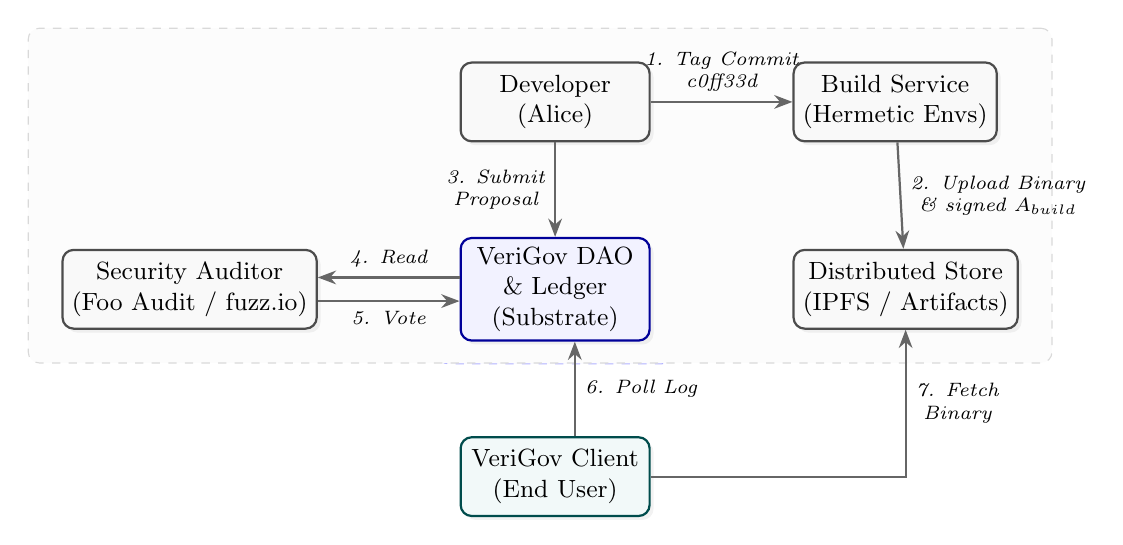
\begin{tikzpicture}[
    node distance=1.2cm and 1.8cm,
    box/.style={draw, rectangle, rounded corners, minimum width=2.4cm, minimum height=1.0cm, align=center, fill=white, drop shadow={opacity=0.1, shadow xshift=0.05cm, shadow yshift=-0.05cm}, font=\small},
    ledger/.style={box, fill=blue!5!white, draw=blue!60!black, thick},
    component/.style={box, fill=gray!5!white, draw=gray!60!black, thick},
    user/.style={box, fill=teal!5!white, draw=teal!60!black, thick},
    arrow/.style={-Stealth, thick, draw=gray!80!black},
    label/.style={font=\scriptsize\itshape, align=center}
  ]
    % Nodes
    \node[component] (dev) {Developer\\(Alice)};
    \node[component, right=of dev] (build) {Build Service\\(Hermetic Envs)};
    
    \node[ledger, below=of dev] (ledger) {VeriGov DAO\\\& Ledger\\(Substrate)};
    \node[component, right=of ledger] (ipfs) {Distributed Store\\(IPFS / Artifacts)};
    \node[component, left=of ledger] (auditor) {Security Auditor\\(Foo Audit / fuzz.io)};
    
    \node[user, below=of ledger] (client) {VeriGov Client\\(End User)};

    % Connections
    \draw[arrow] (dev) -- node[label, above] {1. Tag Commit\\c0ff33d} (build);
    \draw[arrow] (build) -- node[label, right] {2. Upload Binary\\\& signed $A_{build}$} (ipfs);
    \draw[arrow] (dev) -- node[label, left] {3. Submit\\Proposal} (ledger);
    
    % Read & Vote (Auditor)
    \draw[arrow] ($(ledger.west)+(0,0.15)$) -- node[label, above] {4. Read} ($(auditor.east)+(0,0.15)$);
    \draw[arrow] ($(auditor.east)+(0,-0.15)$) -- node[label, below] {5. Vote} ($(ledger.west)+(0,-0.15)$);
    
    % Client verification
    \draw[arrow] ($(client.north)+(0.25,0)$) -- node[label, right] {6. Poll Log} ($(ledger.south)+(0.25,0)$);
    \draw[arrow] (client.east) -| node[label, pos=0.75, right] {7. Fetch\\Binary} (ipfs.south);

    % Background Fit groups
    \begin{scope}[on background layer]
      \node[draw=blue!30, dashed, fill=blue!2!white, rounded corners, fit=(ledger), inner sep=8pt, label={[font=\footnotesize\bfseries, blue!80!black]above:On-Chain}] (onchain) {};
      \node[draw=gray!30, dashed, fill=gray!2!white, rounded corners, fit=(dev) (build) (ipfs) (auditor), inner sep=12pt, label={[font=\footnotesize\bfseries, gray!80!black]above:Off-Chain Ecosystem}] (offchain) {};
    \end{scope}

  \end{tikzpicture}
  \caption{VeriGov Protocol Architecture and Operational Flows. Highlighting the separation between off-chain artifact storage, independent rebuild auditing, and the on-chain consensus-enforced release log.}
  \label{fig:architecture}
\end{figure}


\subsection{Cryptographic Attestation of Source-to-Binary Provenance}

A cornerstone of VeriGov is the ability to cryptographically prove that a binary was created from a specific version of the source code. This is achieved through a verifiable build process and a resulting build attestation.

\begin{itemize}
\item \textbf{The Verifiable Build Process:} We define a build as verifiable if it is both \emph{reproducible} and \emph{attested}. To achieve this, the build must be performed in a \emph{hermetic} environment, meaning it is isolated from the network and has no access to external resources beyond a precisely defined set of dependencies.~\cite{lamb2022reproducible} This is typically accomplished using containerization technologies like Docker. The build environment itself (the container image) must be versioned and its hash recorded to ensure the build can be reproduced by anyone.
\item \textbf{The Build Attestation (}$A_{build}$\textbf{):} This is the data structure that captures the proof of provenance. It is a JSON object that is digitally signed by the build service that performed the compilation.~\cite{slsa} This attestation is then stored in the Distributed Artifact Store, and its hash is included in the release proposal on the VeriGov Ledger. The structure of $A_{build}$ is critical and contains the following fields:
\begin{itemize}
\item \lstinline{source_commit_hash}: The full Git commit hash of the source code version that was checked out for the build.
\item \lstinline{source_tree_hash}: The cryptographic hash of the entire source code tree at that commit. This protects against any modifications to the source after the commit was made.
\item \lstinline{build_environment_hash}: The digest (hash) of the container image or a hash of the complete build environment configuration. This ensures that the same toolchain, system libraries, and dependencies are used for verification builds.~\cite{lamb2022reproducible}
\item \lstinline{output_binary_hash}: The cryptographic hash (e.g., sha256) of the final binary artifact, $H(B)$.
\item \lstinline{builder_signature}: The entire JSON object containing the above fields is signed by the build service's private key.
\end{itemize}
\end{itemize}

This attestation creates a verifiable chain of trust. Any stakeholder or end-user can verify the provenance of a binary by fetching the source code specified by \lstinline{source_commit_hash}, running the build process inside the container specified by \lstinline{build_environment_hash}, and confirming that the hash of their resulting binary matches the \lstinline{output_binary_hash} in the attestation. This process leverages established concepts from the reproducible builds community and the formalisms of cryptographic attestation.~\cite{lamb2022reproducible}

\subsection{Bootstrapping and Cross-Project Trust}
\label{sec:bootstrap}

Two architectural questions deserve explicit treatment before we evaluate VeriGov against existing frameworks: how a project's governance is initiated, and how multiple projects share the protocol.

\paragraph{Genesis state and project registration.} A project joins the VeriGov ecosystem by posting a \texttt{ProjectGenesis} transaction that contains: (i)~a unique project identifier; (ii)~a list of initial stakeholder public keys with their roles; (iii)~the initial role policy (quorums $\{\tau_r\}$ and required-role set $\mathcal{R}_{\text{req}}$); (iv)~the slashing parameters $(\sigma_{\text{neg}}, \sigma_{\text{mal}}, \Delta_{\max})$; and (v)~an initial stake escrow per stakeholder. The genesis transaction is itself signed by the founding maintainer set and is the project's irreducible root of trust---analogous in spirit to TUF's offline Root key, but recorded immutably on-chain so that the entire history of stakeholder evolution is publicly auditable from the project's first moment. From genesis onwards, every change to the stakeholder set or policy must pass a meta-governance proposal (Section~\ref{sec:the-verigov-dao-governance-and-tokenomics}).

\paragraph{Cross-project trust and shared security.} Each project maintains its own stakeholder set, release log, and policy: there is no global ``maintainer of all software.'' However, VeriGov uses a \emph{single, global \texttt{VGOV} token} across all projects rather than per-project tokens. This choice is deliberate. A unified token means that (i)~the same liquid market price $p$ secures every project's economic argument (Equation~\ref{eq:cost}); (ii)~a stakeholder active in multiple projects cannot evade slashing in one by hoarding tokens of another; and (iii)~the protocol's treasury, audit-funding bounties, and governance-of-the-protocol-itself remain coherent. The trade-off is that small projects inherit the price volatility of the broader ecosystem; we view this as a feature, not a bug, since it concentrates economic security where the bulk of the token holders live.

\paragraph{End-user root-of-trust selection.} The end user still faces a one-time choice of which project's release log to trust---installing software requires having a project identifier in mind. This is no worse than today, where users implicitly trust npm/PyPI/GitHub; VeriGov's contribution is that, once a project has been chosen, every subsequent update is verified against an on-chain, multi-stakeholder, economically-bonded approval rather than a single signature.

\subsection{Table 1: Comparison of Software Update Security Frameworks}

To clearly position VeriGov's contributions relative to existing solutions, the following table provides a comparative analysis based on key security features.

\begin{table}[H]
    \centering
    \caption{Security Feature Comparison: Checksum/GPG, TUF, Sigstore, and VeriGov}
    \label{tab:security_comparison}
    \small % Reducing font size slightly to fit the dense content comfortably
    \begin{tabularx}{\textwidth}{>{\bfseries}L L L L L}
        \toprule
        \textbf{Feature} & \textbf{Checksum/GPG} & \textbf{TUF} & \textbf{Sigstore} & \textbf{VeriGov} \\
        \midrule
        Protection Against Transit Errors & Yes (Checksum) & Yes & Yes & Yes \\
        \addlinespace
        Protection Against Rollback/Freeze Attacks & No & Yes (Timestamp/Snapshot roles) & Partial (via Rekor log) & Yes (via immutable ledger) \\
        \addlinespace
        Source-to-Binary Provenance & No & No & No & \textbf{Yes (Cryptographic Build Attestation)} \\
        \addlinespace
        Authenticates Signer Identity & Yes (GPG) & Yes (Key-based roles) & \textbf{Yes (OIDC-based identity)} & Yes (Public key identity) \\
        \addlinespace
        Decentralized Release Authorization & No (Single signer) & No (Centralized Root role) & No (Implicit single-signer policy) & \textbf{Yes ($m$-of-$n$ on-chain voting)} \\
        \addlinespace
        Transparent Governance/Auditability & No & No (Governance is off-band) & Partial (Signing acts are public) & \textbf{Yes (All governance actions are on-chain)} \\
        \addlinespace
        Resilience to Single Maintainer Compromise/Protestware & No & Partial (if Root role is multi-sig) & No & \textbf{Yes (Collective approval required)} \\
        \addlinespace
        Dynamic Stakeholder Management & No (Manual key management) & No (Root role update is off-band) & No & \textbf{Yes (On-chain meta-governance)} \\
        \addlinespace
        Crypto-Economic Security (Incentives/Penalties) & No & No & No & \textbf{Yes (Staking, Rewards, Slashing)} \\
        \bottomrule
    \end{tabularx}
\end{table}

\section{The VeriGov DAO: Governance and Tokenomics}
\label{sec:the-verigov-dao-governance-and-tokenomics}

The heart of the VeriGov protocol is its on-chain governance framework, which formalizes and enforces decision-making processes as a Decentralized Autonomous Organization (DAO).~\cite{dupont2017dao} This approach transforms software release management from an opaque, centralized process into a transparent, community-driven system governed by token holders and executed by immutable smart contracts.~\cite{dupont2017dao} This protocol draws direct inspiration from the sophisticated on-chain governance system of Polkadot, known as OpenGov, which is designed to enable forkless, community-driven network upgrades.~\cite{wood2016polkadot} We adapt its core concepts to the specific domain of software supply chain management.

\subsection{Stakeholders and Roles}

In the VeriGov ecosystem, every participant with governance rights is a stakeholder, represented by an on-chain identity which is cryptographically secured by a public/private key pair. To allow for flexible and secure policies, the framework implements a role-based system. While the specific roles can be customized by each project, a typical configuration might include:

\begin{itemize}
\item \textbf{Core Developer:} These are the primary contributors to the project. Stakeholders with this role are granted the permission to submit New Release proposals to the ledger.
\item \textbf{Security Auditor:} This role is assigned to individuals, trusted security firms, or automated analysis services responsible for vetting the code for vulnerabilities. Their vote may be a mandatory requirement for a release to be approved. In principle, automated agents (e.g., static analysis or fuzzing services) could also hold this role; we discuss the open problems this raises---automated false-positives, prompt injection on source code, and the oracle problem of trusting an automated verdict---in Section~\ref{sec:conclusion-and-future-work}.
\item \textbf{Community Trustee:} These are stakeholders elected by the broader user community to represent their interests in the governance process. This role ensures that decisions are not made solely by the development team and provides a mechanism for user oversight.
\item \textbf{Build Service:} This is a non-human, automated stakeholder. Its role is to perform the verifiable build, generate the \lstinline{A_build} attestation, and publish it to the Distributed Artifact Store. Its signature on the attestation provides the crucial link in the provenance chain.
\end{itemize}

\subsection{The Release Lifecycle (On-Chain Process)}

A new software release progresses through a transparent and verifiable lifecycle, with each step recorded as a transaction on the VeriGov Ledger.

\begin{enumerate}
\item \textbf{Proposal Submission:} A stakeholder with the \lstinline{Core Developer} role initiates the process by submitting a \lstinline{New Release} proposal transaction. This transaction does not contain the binary itself but rather the essential metadata required for verification and voting. The payload includes the proposed version number, the \lstinline{source_commit_hash} from the project's Git repository, and the content hash of the corresponding \lstinline{A_build} attestation (which has already been generated by a \lstinline{Build Service} and stored in the artifact store).
\item \textbf{Verification Phase:} Upon submission, the proposal enters a predefined voting period. This phase triggers an off-chain verification process by all voting stakeholders. They are automatically notified of the new proposal and perform their designated duties:

\begin{itemize}
\item Security auditors review the source code identified by the \lstinline{source_commit_hash} for security vulnerabilities.
\item Other developers perform code reviews for quality and correctness.
\item Crucially, any stakeholder can (and auditors are expected to) independently perform the verifiable build. They fetch the source code, use the specified build environment, and verify that the hash of their locally produced binary matches the \lstinline{output_binary_hash} contained within the \lstinline{A_build} attestation. This step independently confirms the integrity of the build process.
\end{itemize}
\end{enumerate}

\begin{enumerate}\setcounter{enumi}{2}
\item \textbf{Voting:} Stakeholders cast a vote by signing a message $(\text{proposal\_id}, \text{output\_binary\_hash}, \text{yes/no})$ and submitting it as a \texttt{Vote} transaction. We now state the acceptance rule precisely. Let $\mathcal{R}$ be the set of roles defined for the project, $\mathcal{R}_{\text{req}} \subseteq \mathcal{R}$ the subset of roles whose approval is required, $S_r$ the set of stakeholders holding role $r$, $\text{stake}(i)$ the amount of \texttt{VGOV} staked by stakeholder $i$ at the proposal's enactment block, and $\tau_r \in [0,1]$ the project-defined quorum for role $r$. A proposal is accepted if and only if the stake-weighted approval within \emph{every} required role meets its quorum:
\begin{equation}
\forall r \in \mathcal{R}_{\text{req}}: \quad \frac{\sum_{i \in S_r,\, v_i = \text{yes}} \text{stake}(i)}{\sum_{i \in S_r} \text{stake}(i)} \;\geq\; \tau_r.
\label{eq:acceptance}
\end{equation}
Equation~\ref{eq:acceptance} unifies the two governance regimes the protocol blends: the role partition encodes the multi-stakeholder structure ($m$-of-$n$ across roles), while stake weighting within each role aligns voting influence with economic commitment.~\cite{lalley2018qv} Setting $\text{stake}(i)$ to a constant within a role recovers pure $m$-of-$n$ voting; setting $|\mathcal{R}_{\text{req}}|=1$ and pooling all stakeholders into a single role recovers pure stake-weighted voting.

\item \textbf{Tallying and Enactment:} A smart contract on the VeriGov Ledger serves as the automated and impartial tallying mechanism, continuously evaluating Equation~\ref{eq:acceptance} for each active proposal against the project's pre-configured release policy. A typical policy might require, for example, $\tau_{\text{Core Dev}} = 3/5$ and $\tau_{\text{Sec Auditor}} = 1/2$ (with equal stake within each role). Once the policy is satisfied, the contract records the \texttt{output\_binary\_hash} from the successful proposal into the canonical, append-only Official Release Log. From this moment on, VeriGov Clients worldwide will recognize this binary hash as a trusted and valid update.
\end{enumerate}

\begin{figure}[H]
  \centering
  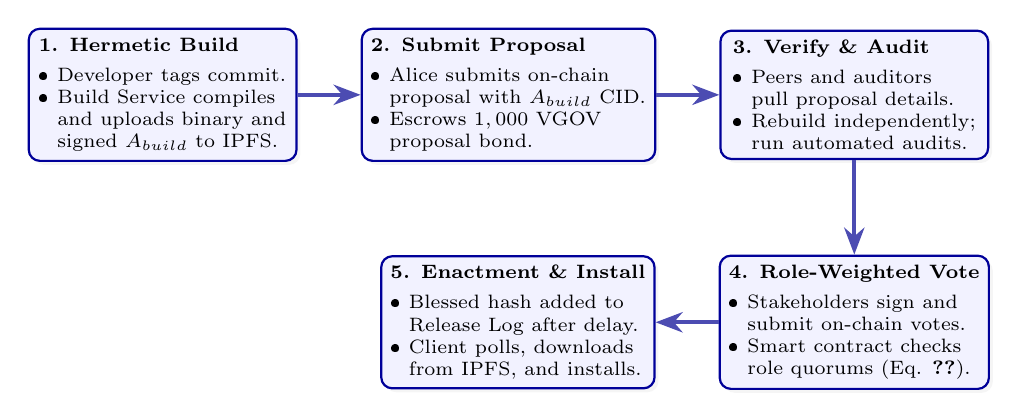
\begin{tikzpicture}[
    stepbox/.style={draw, rectangle, rounded corners, minimum width=3.4cm, minimum height=1.6cm, align=left, fill=white, drop shadow={opacity=0.08, shadow xshift=0.05cm, shadow yshift=-0.05cm}, font=\scriptsize},
    active/.style={stepbox, fill=blue!5!white, draw=blue!60!black, thick},
    arrow/.style={-Stealth, line width=1.5pt, draw=blue!40!gray}
  ]
    % Nodes (Row 1)
    \node[active] (step1) at (0,0) {
      \textbf{1. Hermetic Build}\\[0.1cm]
      \textbullet{} Developer tags commit.\\
      \textbullet{} Build Service compiles\\
      \hphantom{\textbullet{}} and uploads binary and\\
      \hphantom{\textbullet{}} signed $A_{build}$ to IPFS.
    };
    
    \node[active, right=0.8cm of step1] (step2) {
      \textbf{2. Submit Proposal}\\[0.1cm]
      \textbullet{} Alice submits on-chain\\
      \hphantom{\textbullet{}} proposal with $A_{build}$ CID.\\
      \textbullet{} Escrows $1,000$ VGOV\\
      \hphantom{\textbullet{}} proposal bond.
    };
    
    \node[active, right=0.8cm of step2] (step3) {
      \textbf{3. Verify \& Audit}\\[0.1cm]
      \textbullet{} Peers and auditors\\
      \hphantom{\textbullet{}} pull proposal details.\\
      \textbullet{} Rebuild independently;\\
      \hphantom{\textbullet{}} run automated audits.
    };
    
    % Nodes (Row 2)
    \node[active, below=1.2cm of step3] (step4) {
      \textbf{4. Role-Weighted Vote}\\[0.1cm]
      \textbullet{} Stakeholders sign and\\
      \hphantom{\textbullet{}} submit on-chain votes.\\
      \textbullet{} Smart contract checks\\
      \hphantom{\textbullet{}} role quorums (Eq. \ref{eq:acceptance}).
    };
    
    \node[active, left=0.8cm of step4] (step5) {
      \textbf{5. Enactment \& Install}\\[0.1cm]
      \textbullet{} Blessed hash added to\\
      \hphantom{\textbullet{}} Release Log after delay.\\
      \textbullet{} Client polls, downloads\\
      \hphantom{\textbullet{}} from IPFS, and installs.
    };

    % Connections
    \draw[arrow] (step1) -- (step2);
    \draw[arrow] (step2) -- (step3);
    \draw[arrow] (step3) -- (step4);
    \draw[arrow] (step4) -- (step5);

  \end{tikzpicture}
  \caption{VeriGov Software Release Lifecycle. Illustrating the step-by-step pipeline from developer commit to automated build, on-chain proposal, multi-party parallel audit, role-weighted consensus voting, and automated end-user deployment.}
  \label{fig:lifecycle}
\end{figure}


\subsection{Meta-Governance: Evolving the Trust Fabric}

A static set of stakeholders is brittle and cannot adapt to the changing dynamics of a project. People join and leave projects, and trust can be gained or lost. Therefore, the VeriGov protocol includes mechanisms for "meta-governance"---the ability for the stakeholders to govern themselves.

\begin{itemize}
\item \textbf{Add Stakeholder Proposal:} Introducing a new voting member into the trust fabric is a highly sensitive operation. An Add Stakeholder proposal, which nominates a new public key for a specific role, must be subject to a significantly higher voting threshold, such as a super-majority (e.g., two-thirds) of all existing stakeholders. This makes it difficult for a small faction to collude and inject a malicious or controlled voter into the system.
\item \textbf{Remove Stakeholder Proposal:} Conversely, the ability to remove a stakeholder who has been compromised, has lost their keys, or has acted maliciously must be swift. A Remove Stakeholder proposal might therefore have a lower threshold (e.g., a simple majority) to enable the community to react quickly to threats and maintain the integrity of the governance body.~\cite{wright2015decentralized}
\end{itemize}

This on-chain management of the stakeholder set is a critical feature that distinguishes VeriGov from frameworks like TUF, where changes to the root of trust are manual, opaque, and off-band.

\subsection{Tokenomics and Economic Incentives}

The security and sustainability of the VeriGov protocol are underpinned by its native utility token, \lstinline{VGOV}. The tokenomics are designed to create a robust crypto-economic system that aligns the incentives of all participants with the long-term security of the software supply chain.~\cite{saleh2021blockchain}

\subsubsection{Token Utility}

The \lstinline{VGOV} token serves several critical functions within the ecosystem:

\begin{itemize}
\item \textbf{Governance:} \lstinline{VGOV} tokens are required to participate in the DAO's governance. The weight of a stakeholder's vote is proportional to the amount of \lstinline{VGOV} they have staked, ensuring that those with the most significant economic commitment have a corresponding level of influence over the protocol's direction.~\cite{lalley2018qv}
\item \textbf{Staking and Security:} To participate in governance (i.e., to propose or vote on releases), stakeholders must lock up, or "stake," a certain amount of \lstinline{VGOV} tokens. This stake acts as a security deposit or economic bond, which can be forfeited if the stakeholder acts maliciously.~\cite{buterin2017casper}
\item \textbf{Incentive Alignment and Rewards:} The protocol rewards honest and beneficial behavior. A portion of the protocol's revenue (e.g., from transaction fees or a pre-defined inflation schedule) is distributed as rewards to stakeholders who participate correctly in the governance process, such as proposing and voting for releases that are successfully verified and widely adopted.~\cite{buterin2017casper}
\item \textbf{Bounties and Funding:} The VeriGov DAO can maintain a treasury funded by protocol fees. \lstinline{VGOV} token holders can vote to allocate these funds to initiatives that benefit the ecosystem, such as funding security audits, paying for development of new features, or offering bounties for the discovery of vulnerabilities in proposed software.~\cite{dupont2017dao}
\end{itemize}

\subsubsection{Slashing: A Crypto-Economic Disincentive}

The most potent security feature of the VeriGov tokenomic model is \textbf{slashing}: programmatically destroying a portion of a stakeholder's staked tokens in response to provably-bad behavior.~\cite{buterin2017casper} VeriGov adapts this primitive to release governance, but distinguishes two qualitatively different conditions that trigger it.

\paragraph{Negligence slashing.} A negligence offense is one that is \emph{cryptographically self-evident} and adjudicated by the chain itself, without external evidence. The canonical example is a \texttt{Build Service} signing a $A_{build}$ attestation whose \texttt{output\_binary\_hash} does not match the result of an independent reproducible rebuild submitted by another stakeholder. Any party may submit such a counter-attestation as a slashing transaction; if the smart contract verifies the discrepancy, the offending build service's stake is automatically slashed. Negligence slashing also covers double-signing (signing two conflicting votes for the same proposal), signing votes after one's role has been revoked, and missing a sufficiently large fraction of votes (a liveness fault).

\paragraph{Malice slashing.} A malice offense is one that requires \emph{off-chain evidence}---the discovery, days or months after release, that a binary on the Official Release Log is malicious. Because the predicate ``binary $B$ is malicious'' is not a cryptographic relation, malice slashing cannot be fully on-chain. Instead, VeriGov defines a separate \emph{Dispute proposal} track with the following properties: (i)~the challenger posts a substantial bond $b$ in \texttt{VGOV}, forfeit on a frivolous challenge; (ii)~the dispute is decided by a high-quorum vote of stakeholders \emph{who did not vote on the original release proposal} (avoiding the obvious circularity of having the accused vote on their own guilt); (iii)~the dispute window has a configurable statute of limitations $\Delta_{\max}$; (iv)~successful disputes slash the original yes-voters in proportion to their stake and reward the challenger from the slashed pool; (v)~unsuccessful disputes burn the challenger's bond. A diligent voter who reviewed in good faith and was nonetheless fooled by a sufficiently subtle backdoor (xz-style) is still slashed, but at a reduced rate $\sigma_{\text{neg}} < \sigma_{\text{mal}}$ if they participated in the verifiable rebuild and signed the attestation accordingly. This preserves the incentive to participate while still penalizing approval of malware.

\subsubsection{Economic Security: A Cost-of-Attack Lower Bound}
\label{sec:econ-security}

The crypto-economic argument can be quantified. Consider an adversary attempting to push a malicious release. By Equation~\ref{eq:acceptance}, they must obtain ``yes'' votes whose stake-weighted fraction in every required role meets the quorum. Let $\mathcal{R}_{\text{req}} = \{r_1, \dots, r_k\}$ and let $T_r = \tau_r \cdot \sum_{i \in S_r} \text{stake}(i)$ be the minimum stake mass needed in role $r$. For each compromised stakeholder, the adversary either purchases their cooperation (a bribe $\beta_i$) or compromises their key (an offensive-security cost $\kappa_i$). At the malice slashing rate $\sigma_{\text{mal}} \in (0, 1]$, every cooperating stakeholder forfeits $\sigma_{\text{mal}} \cdot \text{stake}(i) \cdot p$, where $p$ is the \texttt{VGOV} unit price at slashing time. A risk-neutral rational adversary therefore faces a cost lower-bounded by
\begin{equation}
C_{\text{attack}} \;\geq\; \sum_{r \in \mathcal{R}_{\text{req}}}\; \sum_{i \in C_r} \big(\sigma_{\text{mal}} \cdot \text{stake}(i) \cdot p \;+\; \min(\beta_i,\kappa_i)\big),
\label{eq:cost}
\end{equation}
where $C_r \subseteq S_r$ is the minimum cooperating set in role $r$ such that $\sum_{i \in C_r} \text{stake}(i) \geq T_r$. Equation~\ref{eq:cost} makes three security-relevant facts explicit. (i)~Security scales with the \emph{product} of stake-per-stakeholder, slashing fraction, and token price; halving any of these halves the security margin. (ii)~Concentration of stake in few large holders reduces $|C_r|$ and therefore the bribe budget, an argument for either reputation-weighted or quadratic-voting refinements (Section~\ref{sec:conclusion-and-future-work}). (iii)~The model assumes $p$ is stable on the attack timescale; an adversary who can short \texttt{VGOV} before executing the attack effectively reduces $p$ in their cost calculation, motivating long unbonding delays so that slashing is enforced at the post-attack price.

\subsection{Worked Example: Releasing \texttt{acme-utils} v1.2.3}
\label{sec:worked-example}

To make the abstract architecture concrete, we walk through one end-to-end release. Project \texttt{acme-utils} has five Core Developers (Alice, Bob, Carol, Dan, Eve), two Security Auditors (the firm Foo Audit and an automated fuzzing service \texttt{fuzz.io}), and a single Build Service. Its policy requires $\tau_{\text{Core Dev}} = 3/5$ stake-weighted approval and $\tau_{\text{Sec Auditor}} = 1/2$.

\textbf{Step 1: Build (off-chain).} Alice tags commit \texttt{c0ff33d} on \texttt{main}. The Build Service checks out \texttt{c0ff33d}, runs the build inside container image \texttt{deadbeef\dots} (recorded as \texttt{build\_environment\_hash}), produces binary $B$ with $H(B) = \texttt{a1b2\dots}$, signs the resulting $A_{build}$, and pins it to IPFS at CID \texttt{Qm\dots42}.

\textbf{Step 2: Proposal (on-chain).} Alice submits a transaction
\[
\texttt{NewRelease}(\text{project=acme-utils},\;\text{version=1.2.3},\;\text{src=c0ff33d},\;\text{attestation=Qm\dots42})
\]
to the VeriGov Ledger; the runtime auto-stakes 1{,}000 \texttt{VGOV} from Alice as proposal bond.

\textbf{Step 3: Verification (off-chain, parallel).} Bob, Carol, and Foo Audit each independently rebuild from \texttt{c0ff33d} inside the specified container; all three obtain $H(B') = \texttt{a1b2\dots}$, matching the attestation. \texttt{fuzz.io} runs its automated test suite against the source tree and finds no regressions.

\textbf{Step 4: Voting (on-chain).} Bob, Carol, and Dan submit \texttt{Vote(yes)}; Eve abstains; Foo Audit submits \texttt{Vote(yes)}; \texttt{fuzz.io} submits \texttt{Vote(yes)}. Stake-weighted approval is computed at the enactment block.

\textbf{Step 5: Tally and enactment.} The smart contract evaluates Equation~\ref{eq:acceptance}: Core Dev approval is $4/5$ stake-weighted (since stakes are equal here) $\geq 3/5 = \tau_{\text{Core Dev}}$; Sec Auditor approval is $2/2 \geq 1/2 = \tau_{\text{Sec Auditor}}$. The proposal is accepted. The contract appends $H(B) = \texttt{a1b2\dots}$ to \texttt{acme-utils}'s Official Release Log after a 24-hour enactment delay.

\textbf{Step 6: Client install.} A user's VeriGov Client polls the Release Log, observes the new entry, fetches $B$ from IPFS by CID, verifies $H(B) = \texttt{a1b2\dots}$, and installs.

\textbf{Failure case.} Suppose a compromised Build Service had silently injected a malicious payload at Step 1. Bob's independent rebuild at Step 3 would yield $H(B') \neq \texttt{a1b2\dots}$. Bob submits a counter-attestation; the negligence-slashing contract verifies the discrepancy and slashes the Build Service's stake without further governance action (Section~\ref{sec:econ-security}).

\subsection{Table 2: VeriGov Governance Parameters and Actions}

The flexibility of the VeriGov protocol is demonstrated by its ability to define different parameters for different types of governance actions. This allows a project to balance the need for speed with the need for security. This concept of distinct proposal "tracks" is inspired by Polkadot's governance design, which includes mechanisms for handling routine proposals, treasury spending, and emergencies with different rules.~\cite{polkadot-opengov}

\begin{table}[H]
    \centering
    \caption{Governance Proposal Lifecycle and Voting Policies}
    \label{tab:governance_policies}
    \footnotesize % Using smaller font to accommodate seven columns
    \setlength{\tabcolsep}{3pt} % Slighting reducing padding between columns
    \begin{tabularx}{\textwidth}{l L L c c l l}
        \toprule
        \textbf{Proposal Type} & \textbf{Initiator Role(s)} & \textbf{Voting Policy ($m$-of-$n$)} & \textbf{Stake} & \textbf{Slash} & \textbf{Period} & \textbf{Delay} \\
        \midrule
        New Release & Core Developer & 3 of 5 Core Dev \textbf{AND} 1 of 2 Sec Auditor & Yes & High & 7 days & 24 hrs \\
        \addlinespace
        Emergency Patch & Core Dev, Sec Auditor & 2 of 5 Core Dev \textbf{OR} 2 of 2 Sec Auditor & Yes & High & 24 hrs & 1 hr \\
        \addlinespace
        Add Stakeholder & Any stakeholder & 66\% of all stakeholders & Yes & N/A & 14 days & 7 days \\
        \addlinespace
        Remove Stakeholder & Any stakeholder & 51\% of all stakeholders & Yes & N/A & 7 days & 24 hrs \\
        \addlinespace
        Update Params & Any stakeholder & 75\% of all stakeholders & Yes & N/A & 30 days & 14 days \\
        \bottomrule
    \end{tabularx}
\end{table}

This table illustrates how a project can establish a standard, deliberate process for regular releases while also defining an expedited track for critical security patches. It also shows how changes to the governance framework itself---adding or removing members, or changing the voting rules---are subject to the highest levels of scrutiny, requiring broad consensus from the existing stakeholders. This ensures that the system is not only secure in its operation but also resilient in its evolution.

\section{Security Analysis}
\label{sec:security-analysis}

A security framework is only as strong as its ability to withstand known and anticipated threats. This section analyzes VeriGov's resilience against the attack vectors identified in Section 2 and explicitly states the trust assumptions upon which the framework is built.

\subsection{Threat Mitigation Analysis}

We revisit the primary threats to the software supply chain and evaluate how the VeriGov architecture and protocol provide mitigation.

\begin{itemize}
\item \textbf{Compromised Maintainer Account:} In a traditional system, an attacker who steals a maintainer's credentials can unilaterally publish a malicious package.~\cite{aikido2025rand} In VeriGov, this is not possible. A single compromised account can, at worst, \emph{propose} a malicious release. However, this proposal will fail to be enacted because it will not receive the required $m$-of-$n$ signatures from the other, uncompromised stakeholders during the voting phase. The crypto-economic model adds another layer of defense: even if an attacker compromises multiple accounts, they would need to convince the owners to risk their staked \lstinline{VGOV} tokens, which would be slashed if the malicious activity is discovered.~\cite{buterin2017casper}
\item \textbf{Malicious "Protestware":} The case of a legitimate maintainer intentionally creating malicious software like \lstinline{node-ipc}~\cite{cve-2022-23812} is a direct assault on the trust placed in developers. VeriGov mitigates this insider threat through mandatory, collective review and economic consequence. The malicious maintainer can author and propose the destructive code, but it cannot be released without the explicit, staked approval of other stakeholders. The \lstinline{Security Auditor} role is specifically designed for this purpose. Upon discovering the malicious payload, auditors would vote against the release, and the on-chain record of the malicious proposal would serve as grounds for a \lstinline{Remove Stakeholder} vote, permanently revoking the malicious actor's governance rights. The threat of both reputational damage and financial loss via slashing makes such an act prohibitively costly.~\cite{buterin2017casper}
\item \textbf{Build Server Compromise (SolarWinds-style):} This attack vector bypasses source code reviews by injecting malware during compilation. VeriGov directly counters this through the verifiable build and attestation mechanism. If an attacker compromises the official \lstinline{Build Service} and causes it to inject malware, the \lstinline{output_binary_hash} in its generated \lstinline{A_build} will be for the malicious binary. However, when other stakeholders (e.g., security auditors) perform their own independent, reproducible build from the clean source code, their locally generated binary hash will not match the one in the attestation. This cryptographic discrepancy is undeniable proof of tampering. The proposal would be rejected, and an investigation into the build service's integrity would be triggered.
\item \textbf{Dependency Confusion:} This attack vector tricks a build system into fetching a malicious public dependency instead of a private one.~\cite{birsan2021dependency} VeriGov mitigates this at a fundamental level through the requirement for a hermetic and reproducible build environment. The configuration of the build environment---including the specific versions and sources (e.g., pointing exclusively to a private registry) of all dependencies---is captured in the \lstinline{build_environment_hash}.~\cite{lamb2022reproducible} Any attempt to use a different dependency would result in a different environment hash, which would invalidate the build attestation and cause the verification to fail.
\end{itemize}

\subsection{Trust Assumptions}

No security system is absolute. It is crucial to be explicit about the assumptions that underpin VeriGov's security model.

\begin{itemize}
\item \textbf{Cryptography:} We assume the underlying cryptographic primitives---specifically, the hash function (e.g., SHA-256) and the digital signature algorithm (e.g., ECDSA)---are computationally secure and have not been broken.
\item \textbf{Client Security:} The initial installation of the VeriGov Client on the end-user's machine is a critical bootstrapping step. We assume this initial binary is authentic and has not been tampered with. Securing this initial download remains an out-of-band challenge, common to all update systems.
\item \textbf{Stakeholder Non-Collusion \& Economic Rationality:} The core trust assumption of VeriGov is shifted from a single entity to a collective. We assume that a malicious actor cannot compromise or coerce the required threshold ($m$) of stakeholders to collude and approve a malicious release. This assumption is strengthened by the economic model; we assume stakeholders are rational economic actors who will not vote for a malicious proposal if the expected financial loss from being slashed is greater than the potential gain from collusion.~\cite{buterin2017casper}
\item \textbf{Liveness of Stakeholders:} The framework requires that a sufficient number of stakeholders remain active and participate in voting for the governance process to function. A project could become deadlocked if too many stakeholders become inactive or lose their keys.
\end{itemize}

\subsection{Limitations and Future Threats}

\begin{itemize}
\item \textbf{Governance Attacks:} A sufficiently motivated and well-resourced adversary could attempt to subvert the governance model itself. This could involve social engineering, bribery, or simultaneously compromising the systems of multiple stakeholders to gain control of enough keys to meet the voting threshold. The defense against this is a robust and diverse stakeholder set and strong operational security for all participants.
\item \textbf{Release Latency and Throughput:} A 7-day default voting window for a New Release proposal (Table~\ref{tab:governance_policies}) is incompatible with continuous-deployment projects that ship hourly. Three mitigations apply: (i)~\emph{batched releases}, where a single proposal authorizes a range of micro-releases that share a build attestation pattern; (ii)~\emph{delegated pre-approval}, where Core Developers stake-delegate to a smaller signing committee whose decisions are auto-ratified absent challenge within a short window; and (iii)~\emph{adversarial-resistance tracks} that trade voting period for stake bond size. Independent of latency, the underlying ledger's transaction throughput and economic-security properties (e.g., resistance to MEV-style attacks~\cite{daian2020flash}) bound the protocol's practical capacity and must be considered in any implementation.
\item \textbf{The "Trusting Trust" Compiler Attack:} The current framework relies on reproducible builds, which assumes the compiler itself is benign. A highly sophisticated attacker could execute a "Reflections on Trusting Trust" attack by providing a compromised compiler to all stakeholders.~\cite{thompson1984trusting} This malicious compiler could appear to function correctly but subtly inject a backdoor into the compiled binary. Since all stakeholders would be using the same malicious compiler, their reproducible builds would all produce the same malicious binary, and the attack would go undetected. Mitigating this threat requires advancing the state of the art to either use multiple, independently developed compilers for diverse double-compilation~\cite{wheeler2005diverse} or, ideally, a formally verified compiler like CompCert that is mathematically proven to be correct.~\cite{leroy2009compcert}
\end{itemize}

\section{Conclusion and Future Work}
\label{sec:conclusion-and-future-work}

\subsection{Summary of Contributions}

The modern software supply chain is plagued by vulnerabilities stemming from centralized trust models that fail to provide adequate guarantees for either provenance or authorization. Existing solutions like TUF and Sigstore address important but isolated parts of this problem, leaving critical gaps that have been exploited in numerous high-profile attacks. This paper has introduced VeriGov, a holistic, crypto-economic protocol that provides a robust, end-to-end security solution for software distribution and updates.

VeriGov's principal contribution is the unique synthesis of three key security paradigms:

\begin{enumerate}
\item \textbf{Decentralized, On-Chain Governance:} By establishing a DAO and moving release authorization to a public blockchain, VeriGov eliminates the single point of failure inherent in current systems. It provides transparent, auditable, and cryptographically enforced governance, making it resilient to both external attacks on single accounts and internal threats from malicious maintainers.~\cite{wright2015decentralized}
\item \textbf{Verifiable Source-to-Binary Provenance:} Through the use of cryptographic build attestations generated from hermetic and reproducible build environments, VeriGov creates an undeniable link between a software binary and the precise source code that created it. This closes the provenance gap and allows any party to independently verify that a binary has not been tampered with during the build process.~\cite{slsa}
\item \textbf{Crypto-Economic Security:} The introduction of the \lstinline{VGOV} token, with its integrated staking and slashing mechanisms, fundamentally changes the security model. It aligns the financial incentives of all participants with the security of the network, making malicious behavior economically irrational and prohibitively expensive.~\cite{buterin2017casper}
\end{enumerate}

By combining these pillars, VeriGov establishes a new standard for trust in the software supply chain, shifting reliance from fallible human actors and opaque processes to a system of collective responsibility and cryptographic and economic certainty.

\subsection{Future Work}

The conceptual framework presented in this paper lays the groundwork for several promising avenues of future research and development.

\begin{itemize}
\item \textbf{Prototype Implementation:} The immediate next step is to build a proof-of-concept prototype of the VeriGov framework. This could be implemented using an existing blockchain framework like Hyperledger Fabric or Substrate for the VeriGov Ledger, coupled with IPFS for the Distributed Artifact Store. A simple VeriGov Client could be developed to demonstrate the end-to-end workflow of proposing, voting on, and securely installing an update.
\item \textbf{Advanced Tokenomic Models:} The current model uses token-weighted voting. Future work could explore more advanced governance mechanisms to further decentralize power and mitigate the risk of "whales" (large token holders) dominating votes. This includes exploring \textbf{reputation-based governance}, where voting power is influenced by past positive contributions, and \textbf{quadratic voting}, where the cost of each additional vote increases, giving smaller stakeholders a more proportional voice.~\cite{lalley2018qv}
\item \textbf{Formal Verification of the Protocol:} To achieve the highest level of assurance, the VeriGov smart contracts and governance protocols themselves should be formally verified. Using proof assistants like Coq or Isabelle, it would be possible to create a mathematical proof that the protocol correctly implements its specified security properties (e.g., that a release cannot be enacted without meeting the $m$-of-$n$ threshold).~\cite{leroy2009compcert}
\item \textbf{AI-Powered Stakeholders.} A forward-looking research direction is the use of automated agents as Security Auditor stakeholders---running static analysis, fuzzing, or formal verification on a proposal's source tree and casting a vote based on the result. Several non-trivial open problems must be addressed before this is deployable: false-positive rates that would block legitimate releases, prompt-injection attacks where adversarial source code subverts an LLM-based reviewer, the oracle problem of whether a passing test result is itself trustworthy, and the question of how much stake an automated agent should carry given that it cannot be ``slashed for negligence'' in the same human-accountable sense. We see these as a research agenda rather than a near-term feature.
\end{itemize}

\bibliographystyle{IEEEtran}
\bibliography{references}

\end{document}
